

\chapter{Uvod}

	 Cilj ovog projektnog zadatka detaljna je analiza odabranog skupa podataka. Skup podataka čine različiti atributi, a naš je zadatak doći do dubokog razumijevanja njihovih međusobnih odnosa i potencijalnih trendova. Sve to namjeravamo ostvariti kroz proces čišćenja podataka, statističke analize i vizualizacije. Za eksploratornu analizu odabran je podatkovni skup \textit{IMDb movie dataset} koji sadrži informacije o filmovima, uključujući ocjene, godine premijere, glumačku postavu i druge relevantne podatke, prikupljene s popularnog filmskog portala IMDb. Očekujemo da ćemo kroz analizu ovog skupa podataka istražiti i shvatiti karakteristike filmova, odnose između različitih atributa skupa te steći dublji uvid u svijet filmova.
	 
	 \section{Pregled i čišćenje podataka}
	 
	 Originalni skup podata \textit{IMDb movie dataset} sastoji se od ukupno 5043 zapisa s ukupno 28 atributa. Izvođenjem jednostavne naredbe 
	 
	 \lstinputlisting[language=R]{../R/007.R}
	 
	 \noindent utvrđeno je da duplicirani zapisi čine 45 redaka izvornog skupa. Duplicirani su redci izbačeni iz skupa i konačni se skup sastoji od 4998 zapisa. Prije eksportiranja uređenog skupa za daljnje korištenje tijekom analize, zbog lakšeg je snalaženja promijenjen i redoslijed stupaca. Redoslijed stupaca promijenjen je izvršavanjem sljedeće naredbe: 
	 
	 \lstinputlisting[language=R]{../R/008.R}
	 
	 \noindent Imena varijabli i opisi značenja mogu se provjeriti u tablici na web stranici Kaggle\footnote{https://www.kaggle.com/code/harshadeepvattikunta/predicting-movie-success}. Nakon navedenih izmjena, podatkovni je skup spreman za eksportiranje u \texttt{.csv} formatu. Sve daljnje analize provode se nad novodobivenom, \textit{očišćenom}, verzijom skupa podataka.  
	 
	 \section[Osnovne informacije o atributima podatkovnog skupa]{Osnovne informacije o atributima podatkovnog \\ skupa}
	 
	 U ovom ćemo dijelu, s ciljem boljeg upoznavanja sa skupom podatka, provesti jednostavne analize nad podacima svakog stupca zasebno. 
	 
	 Najprije primjenom funkcije \texttt{sapply} saznajemo broj vrijednosti koje nedostaju (\textit{NA} vrijednosti) u svakom stupcu.
	 
	 \begin{table}[H]
	 	\centering
	 	\caption{Broj nepoznatih vrijednosti po stupcu}
	 	\label{missing-values}
	 	\begin{tabular}{|l|c|l|c|}
	 		\hline
	 		\textbf{Stupac} & \textbf{Broj} & \textbf{Stupac} & \textbf{Broj} \\
	 		\hline
	 		\texttt{movie\_title} & 0 & \texttt{num\_user\_for\_reviews} & 21 \\
	 		\hline
	 		\texttt{duration} & 15 & \texttt{num\_critic\_for\_reviews} & 49 \\
	 		\hline
	 		\texttt{director\_name} & 103 & \texttt{num\_voted\_users} & 0 \\
	 		\hline
	 		\texttt{director\_facebook\_likes} & 103 & \texttt{cast\_total\_facebook\_likes} & 0 \\
	 		\hline
	 		\texttt{actor\_1\_name} & 7 & \texttt{movie\_facebook\_likes} & 0 \\
	 		\hline
	 		\texttt{actor\_1\_facebook\_likes} & 7 & \texttt{plot\_keywords} & 152 \\
	 		\hline
	 		\texttt{actor\_2\_name} & 13 & \texttt{facenumber\_in\_poster} & 13 \\
	 		\hline
	 		\texttt{actor\_2\_facebook\_likes} & 13 & \texttt{color} & 19 \\
	 		\hline
	 		\texttt{actor\_3\_name} & 23 & \texttt{genres} & 0 \\
	 		\hline
	 		\texttt{actor\_3\_facebook\_likes} & 23 & \texttt{title\_year} & 107 \\
	 		\hline
	 		\texttt{language} & 12 & \texttt{country} & 5 \\
	 		\hline
	 		\texttt{content\_rating} & 301 & \texttt{aspect\_ratio} & 327 \\
	 		\hline
	 		\texttt{movie\_imdb\_link} & 0 & \texttt{gross} & 874 \\
	 		\hline
	 		\texttt{budget} & 487 & \texttt{imdb\_score} & 0 \\
	 		\hline
	 	\end{tabular}
	 \end{table}
	 
	 Podaci u stupcima s nazivom \texttt{actor\_n\_facebook\_likes}, \texttt{n} $= 1, 2, 3$,  sadrže podatke o broju \textit{lajkova} na Facebook stranici glumca \texttt{actor\_n\_name}, \texttt{n} $= 1, 2, 3$. Izdvajanjem imena glumaca i njihovih odgovarajućih brojeva \texttt{lajkova} te uzimajući u obzir samo najviši broj \textit{lajkova} za pojedinog glumca, dobivamo podatke o najpoznatijim glumcima (najpoznatiji u ovom kontekstu znači s najviše \textit{lajkova}). Imena i broj \textit{lajkova} pet najpoznatijih glumaca navedeni su u tablici \ref{najpoznatiji_glumci}. 
	 
	 
	 \begin{table}[H]
	 	\centering
	 	\renewcommand{\arraystretch}{1.5} % Adjust the value to increase or decrease row spacing
	 	\begin{tabular}{|l|c|}
	 		\hline
	 		\multicolumn{1}{|c|}{\textbf{Ime glumca}} & \multicolumn{1}{c|}{\textbf{Broj Facebook \textit{lajkova}}} \\
	 		\hline
	 		Darcy Donavan & 640,000 \\
	 		\hline
	 		Matthew Ziff & 260,000 \\
	 		\hline			
	 		Krista Allen & 164,000 \\
	 		\hline		
	 		Andrew Fiscella & 137,000 \\
	 		\hline		
	 		Jimmy Bennett & 87,000 \\
	 		\hline
	 	\end{tabular}
	 	\caption{Najpoznatiji glumci}
	 	\label{najpoznatiji_glumci}
	 \end{table}
	 
	 Također, na temelju podataka iz stupaca \texttt{actor\_n\_name}, \texttt{n} $= 1, 2, 3$ te \texttt{director\_name} izdvojili smo glumce i redatelje s najviše filmova. U tablici \ref{glumci_s_najvise_uloga} prikazan je popis 5 glumaca s najviše uloga, dok su u tablici \ref{redatelji_s_najvise_filmova} prikazani redatelji koji su režirali najviše filmova.
	 
	  \begin{table}[H]
	 	\centering
	 	\renewcommand{\arraystretch}{1.5} % Adjust the value to increase or decrease row spacing
	 	\begin{tabular}{|l|c|}
	 		\hline
	 		\multicolumn{1}{|c|}{\textbf{Ime glumca}} & \multicolumn{1}{c|}{\textbf{Broj uloga}} \\
	 		\hline
	 		Robert De Niro & 54 \\
	 		\hline
	 		Morgan Freeman & 47 \\
	 		\hline			
	 		Bruce Willis & 40 \\
	 		\hline		
	 		Johnny Depp & 40 \\
	 		\hline		
	 		Matt Damon	& 38 \\
	 		\hline
	 	\end{tabular}
	 	\caption{Glumci s najviše uloga}
	 	\label{glumci_s_najvise_uloga}
	 \end{table}
	 
	 \begin{table}[H]
	 	\centering
	 	\renewcommand{\arraystretch}{1.5} % Adjust the value to increase or decrease row spacing
	 	\begin{tabular}{|l|c|}
	 		\hline
	 		\multicolumn{1}{|c|}{\textbf{Ime redatelja}} & \multicolumn{1}{c|}{\textbf{Broj režija}} \\
			 \hline
			 Steven Spielberg & 26 \\
			 \hline
			 Woody Allen & 22 \\
			 \hline			
			 Clint Eastwood & 20 \\
			 \hline		
			 Martin Scorsese & 20 \\
			 \hline		
			 Ridley Scott & 17 \\
			 \hline
		 \end{tabular}
		 \caption{Najčešći redatelji}
		 \label{redatelji_s_najvise_filmova}
	 \end{table}
	 
	 Iz podataka sadržanih u stupcu nazvanom \texttt{cast\_total\_facebook\_likes} moguće je  identificirati filmove s najpoznatijom glumačkom postavom, a to su filmovi navedeni u tablici \ref{najpoznatiji_casting}.
	 
	  \begin{table}[H]
	 	\centering
	 	\renewcommand{\arraystretch}{1.5}  
	 	\begin{tabular}{|l|>{\centering\arraybackslash}p{2cm}|>{\centering\arraybackslash}p{2cm}|>{\centering\arraybackslash}p{2.5cm}|}
	 		\hline
	 		\multicolumn{1}{|c|}{\multirow{2}{*}{\textbf{Naslov filma}}} & \textbf{Godina premijere} & \textbf{IMDB ocjena} & \textbf{Broj \textit{lajkova} postave} \\
	 		\hline
	 		Anchorman: The Legend of Ron Burgundy & 2004 & 7.2 & 656,730 \\
	 		\hline
	 		The Final Destination & 2009 & 5.2 & 303,717 \\
	 		\hline
	 		Treachery & 2013 & 3.9 & 283,939 \\
	 		\hline
	 		Hardflip & 2012 & 5.6 & 263,584 \\
	 		\hline
	 		Kickboxer: Vengeance & 2016 & 9.1 & 261,818 \\
	 		\hline
	 	\end{tabular}
	 	\caption{Filmovi s najpoznatijom glumačkom postavom}
	 	\label{najpoznatiji_casting}
	 \end{table}
	 
	 Stupac \texttt{plot\_keywords} sastoji se od ključnih riječi koje opisuju radnju filma odvojenih znakom '$|$'. Razdvajanjem sadržaja stupca po znaku '$|$' izdvajamo pojedinačne ključne riječi i saznajemo koje su najčešće te ih navodimo u tablici \ref{keywords}.
	 
	 \begin{table}[H]
	 	\centering
	 	\renewcommand{\arraystretch}{1.5} % Adjust the value to increase or decrease row spacing
	 	\begin{tabular}{|l|c|l|c|}
	 		\hline
	 		\multicolumn{1}{|c|}{\textbf{Ključna riječ}} & \multicolumn{1}{c|}{\textbf{Broj filmova}} & \multicolumn{1}{c|}{\textbf{Ključna riječ}} & \multicolumn{1}{c|}{\textbf{Broj filmova}} \\
	 		\hline
	 		love & 194 & fbi & 71 \\
	 		\hline
	 		friend & 165 & revenge & 70 \\
	 		\hline
	 		murder & 159 & friendship & 67 \\
	 		\hline
	 		death & 132 & drugs & 66 \\
	 		\hline
	 		police & 126 & prison & 62 \\
	 		\hline
	 		new york city & 91 & money & 61 \\
	 		\hline
	 		high school & 89 & marriage & 60 \\
	 		\hline
	 		alien & 82 & female protagonist & 57 \\
	 		\hline
	 		school & 73 & island & 57\\
	 		\hline
	 		boy & 72 & dog & 56\\
	 		\hline
	 	\end{tabular}
	 	\caption{Najčešće ključne riječi koje opisuju radnju filma}
	 	\label{keywords}
	 \end{table} 
	 
	 Sličan stupcu \texttt{plot\_keywords} stupac je \texttt{genres} koji, odvojene znakom '$|$', sadrži informacije o žanrovima filmova. Izdvajamo žanrove za svaki film i prikazujemo broj filmova po svakom od žanrova u histogramu na slici \ref{filmovi_zanr}.
	 
	 \begin{figure}[H]
	 	\centering
	 	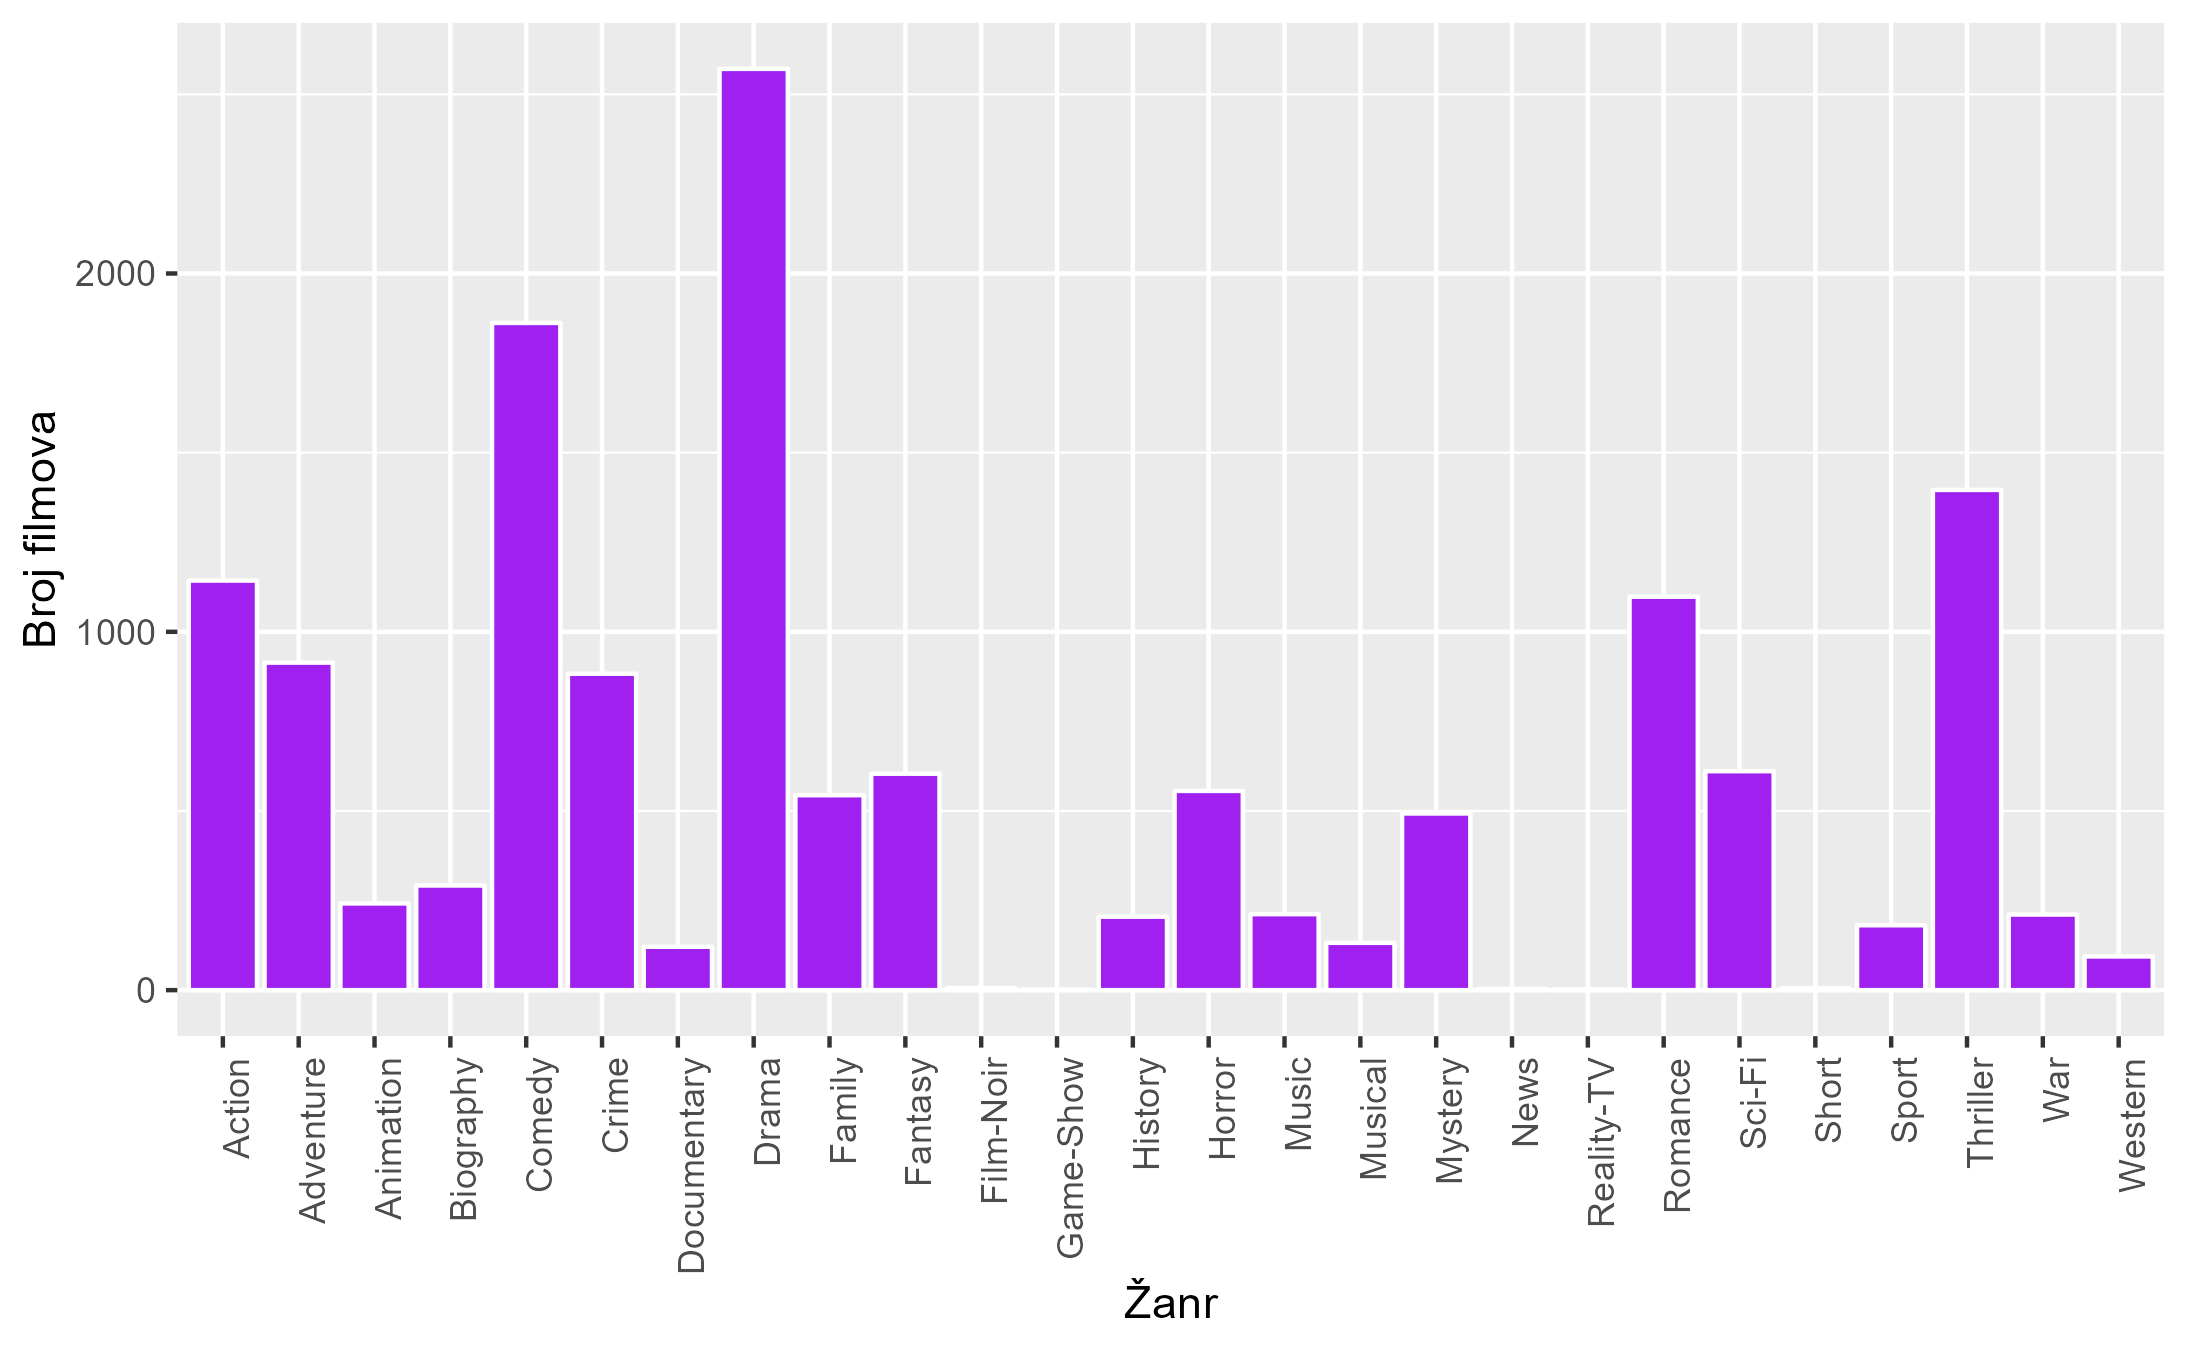
\includegraphics[width=15cm]{../figures/analysis/broj_filmova_po_zanru.png}
	 	\caption{Podjela filmova po žanru}
	 	\label{filmovi_zanr}
	 \end{figure}
	 
	 Stupac \texttt{title\_year} poprima vrijednosti od 1916 do 2016, a predstavlja godinu premijere filma. Koje je godine premijerno prikazano koliko filmova prikazano je na slici \ref{filmovi_godine}.
	 
	  \begin{figure}[H]
	 	\centering
	 	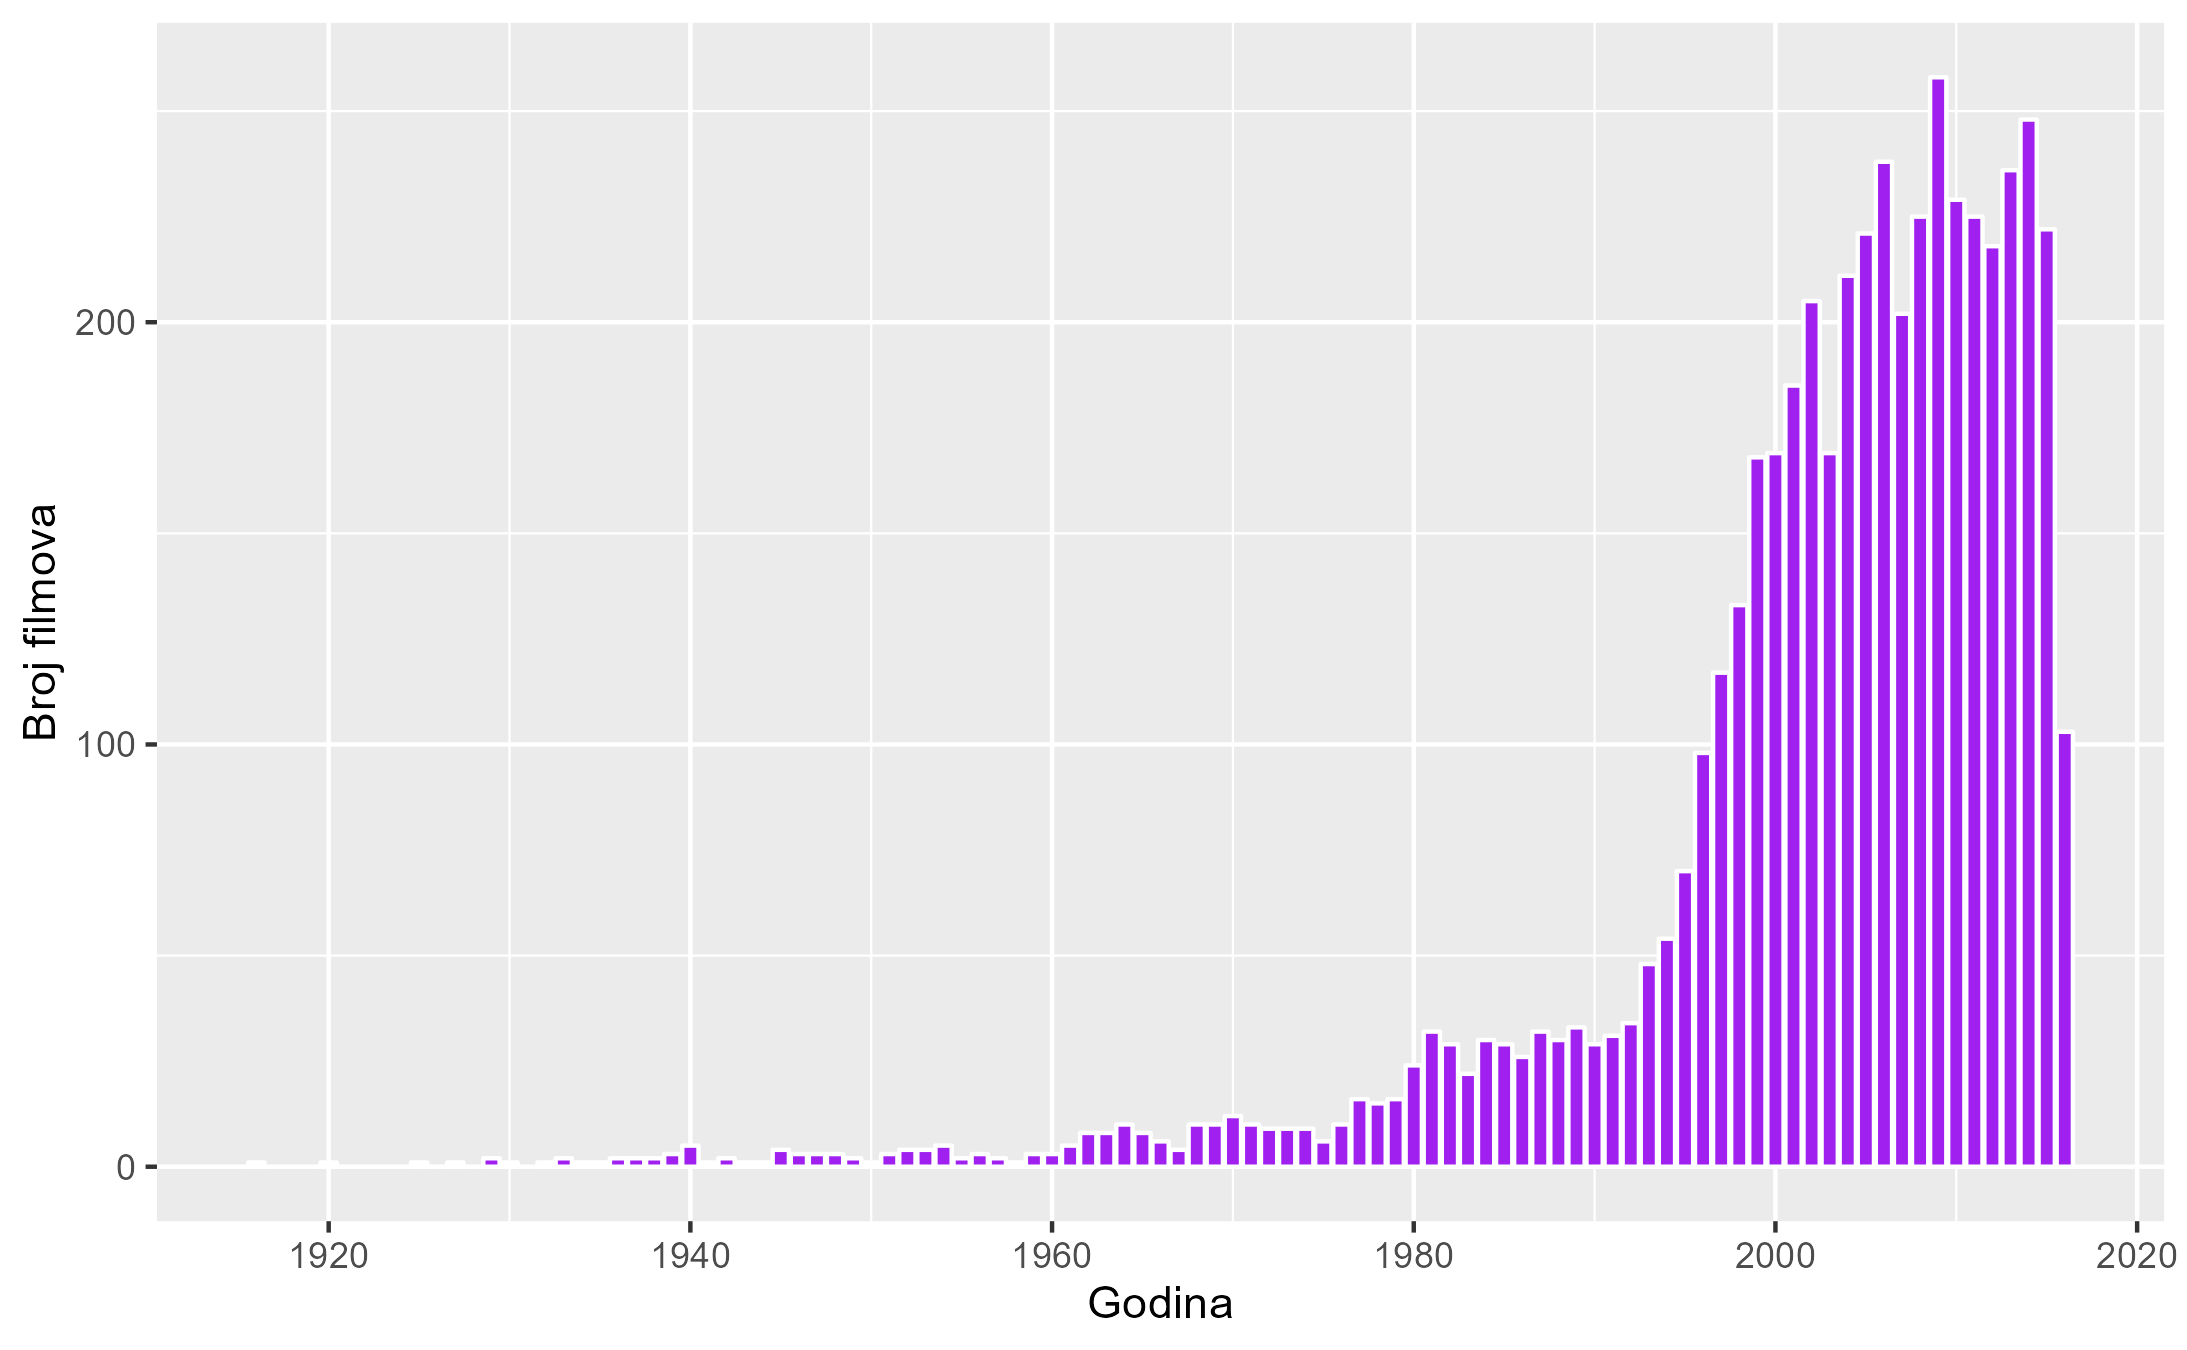
\includegraphics[width=15cm]{../figures/analysis/broj_filmova_po_godini.png}
	 	\caption{Broj filmova po godini premijere}
	 	\label{filmovi_godine}
	 \end{figure}
	 
	 U stupcu \texttt{facenumber\_in\_poster} zapisan je broj glumaca koji se pojavljuju na plakatu filma. Za većinu filmova (njih ukupno 2136) taj je broj nula, a najveći broj glumaca na plakatu iznosi 43 (za film \textit{500 Days of Summer}). Prosječna je vrijednost atributa \texttt{facenumber\_in\_poster} 1.37, a medijan 1.
	 
	 Za koju je dobnu skupinu film namijenjen sadržano je u stupcu \texttt{content\_rating}. Popis najčešćih starosnih ograničenja i njihova značenja dana su u tablici \ref{content_rating}.
	 
	 \begin{table}[H]
	 	\centering
	 	\renewcommand{\arraystretch}{1.5} % Adjust the value to increase or decrease row spacing
	 	\begin{tabular}{|c|c|l|}
	 		\hline
	 		\multicolumn{1}{|c|}{\textbf{Ograničenje}} & \multicolumn{1}{c|}{\textbf{Broj filmova}} & \multicolumn{1}{c|}{\textbf{Značenje}} \\
	 		\hline
	 		R & 2098 & Za osobe starije od 17 godina \\
	 		\hline 
	 		PG-13 & 1444 & Za osobe starije od 13 godina \\
	 		\hline
	 		PG & 688 & Za osobe starije od 8 godina \\
	 		\hline
	 	\end{tabular}
	 	\caption{Najčešća starosna ograničenja filmova}
	 	\label{content_rating}
	 \end{table}
	 
	 Omjer širine i visine (proporcije) filmske slike za pojedini film zapisan je u stupcu \texttt{aspect\_ratio}. U skupu podataka pojavljuje se ukupno 23 različitih omjera, a za sedam najčešćih napravljen je pregled (slika \ref{proporcije}) kretanja broja filmova s tim proporcijama po godinama. 
	 
	  \begin{figure}[H]
	 	\centering
	 	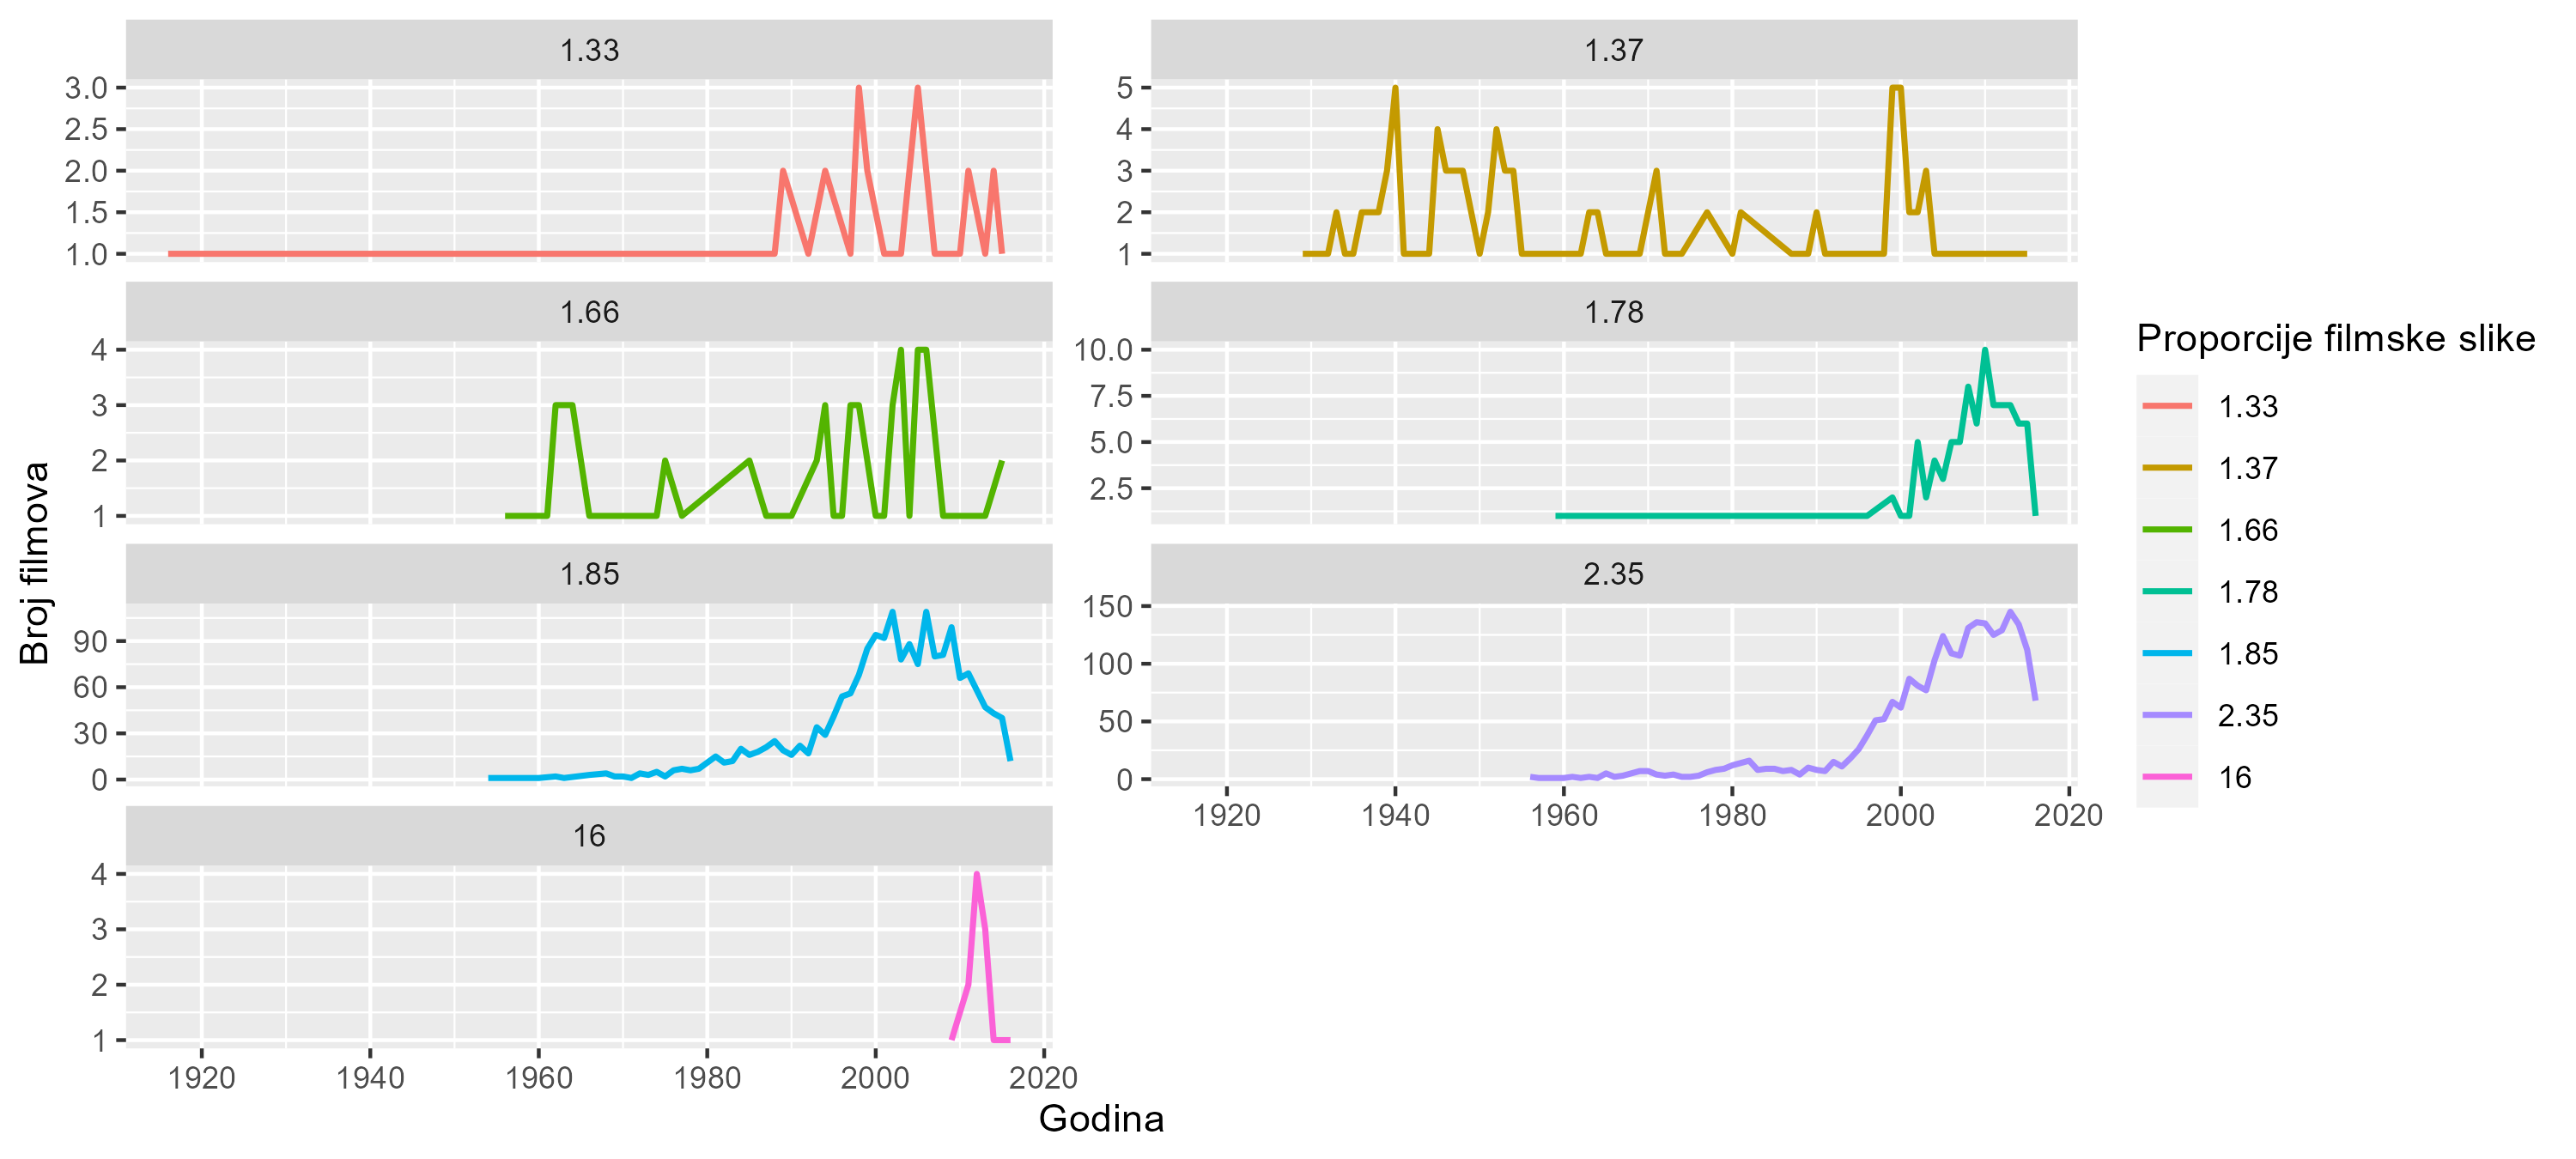
\includegraphics[width=15cm]{../figures/analysis/proporcije_i_godine.png}
	 	\caption{Broj filmova s najčešćim proporcijama filmske slike po godinama }
	 	\label{proporcije}
	 \end{figure}
	 
	 U stupcima \texttt{budget} i \texttt{gross} nalaze se podaci o budžetu filma i ukupnoj bruto zaradi filma u američkim dolarima. Koliki je postotak filmova svake godine ostvario manju zaradu od iznosa budžeta prikazujemo na slici \ref{neuspjesno}.
	 
	 
	 \begin{figure}[H]
	 	\centering
	 	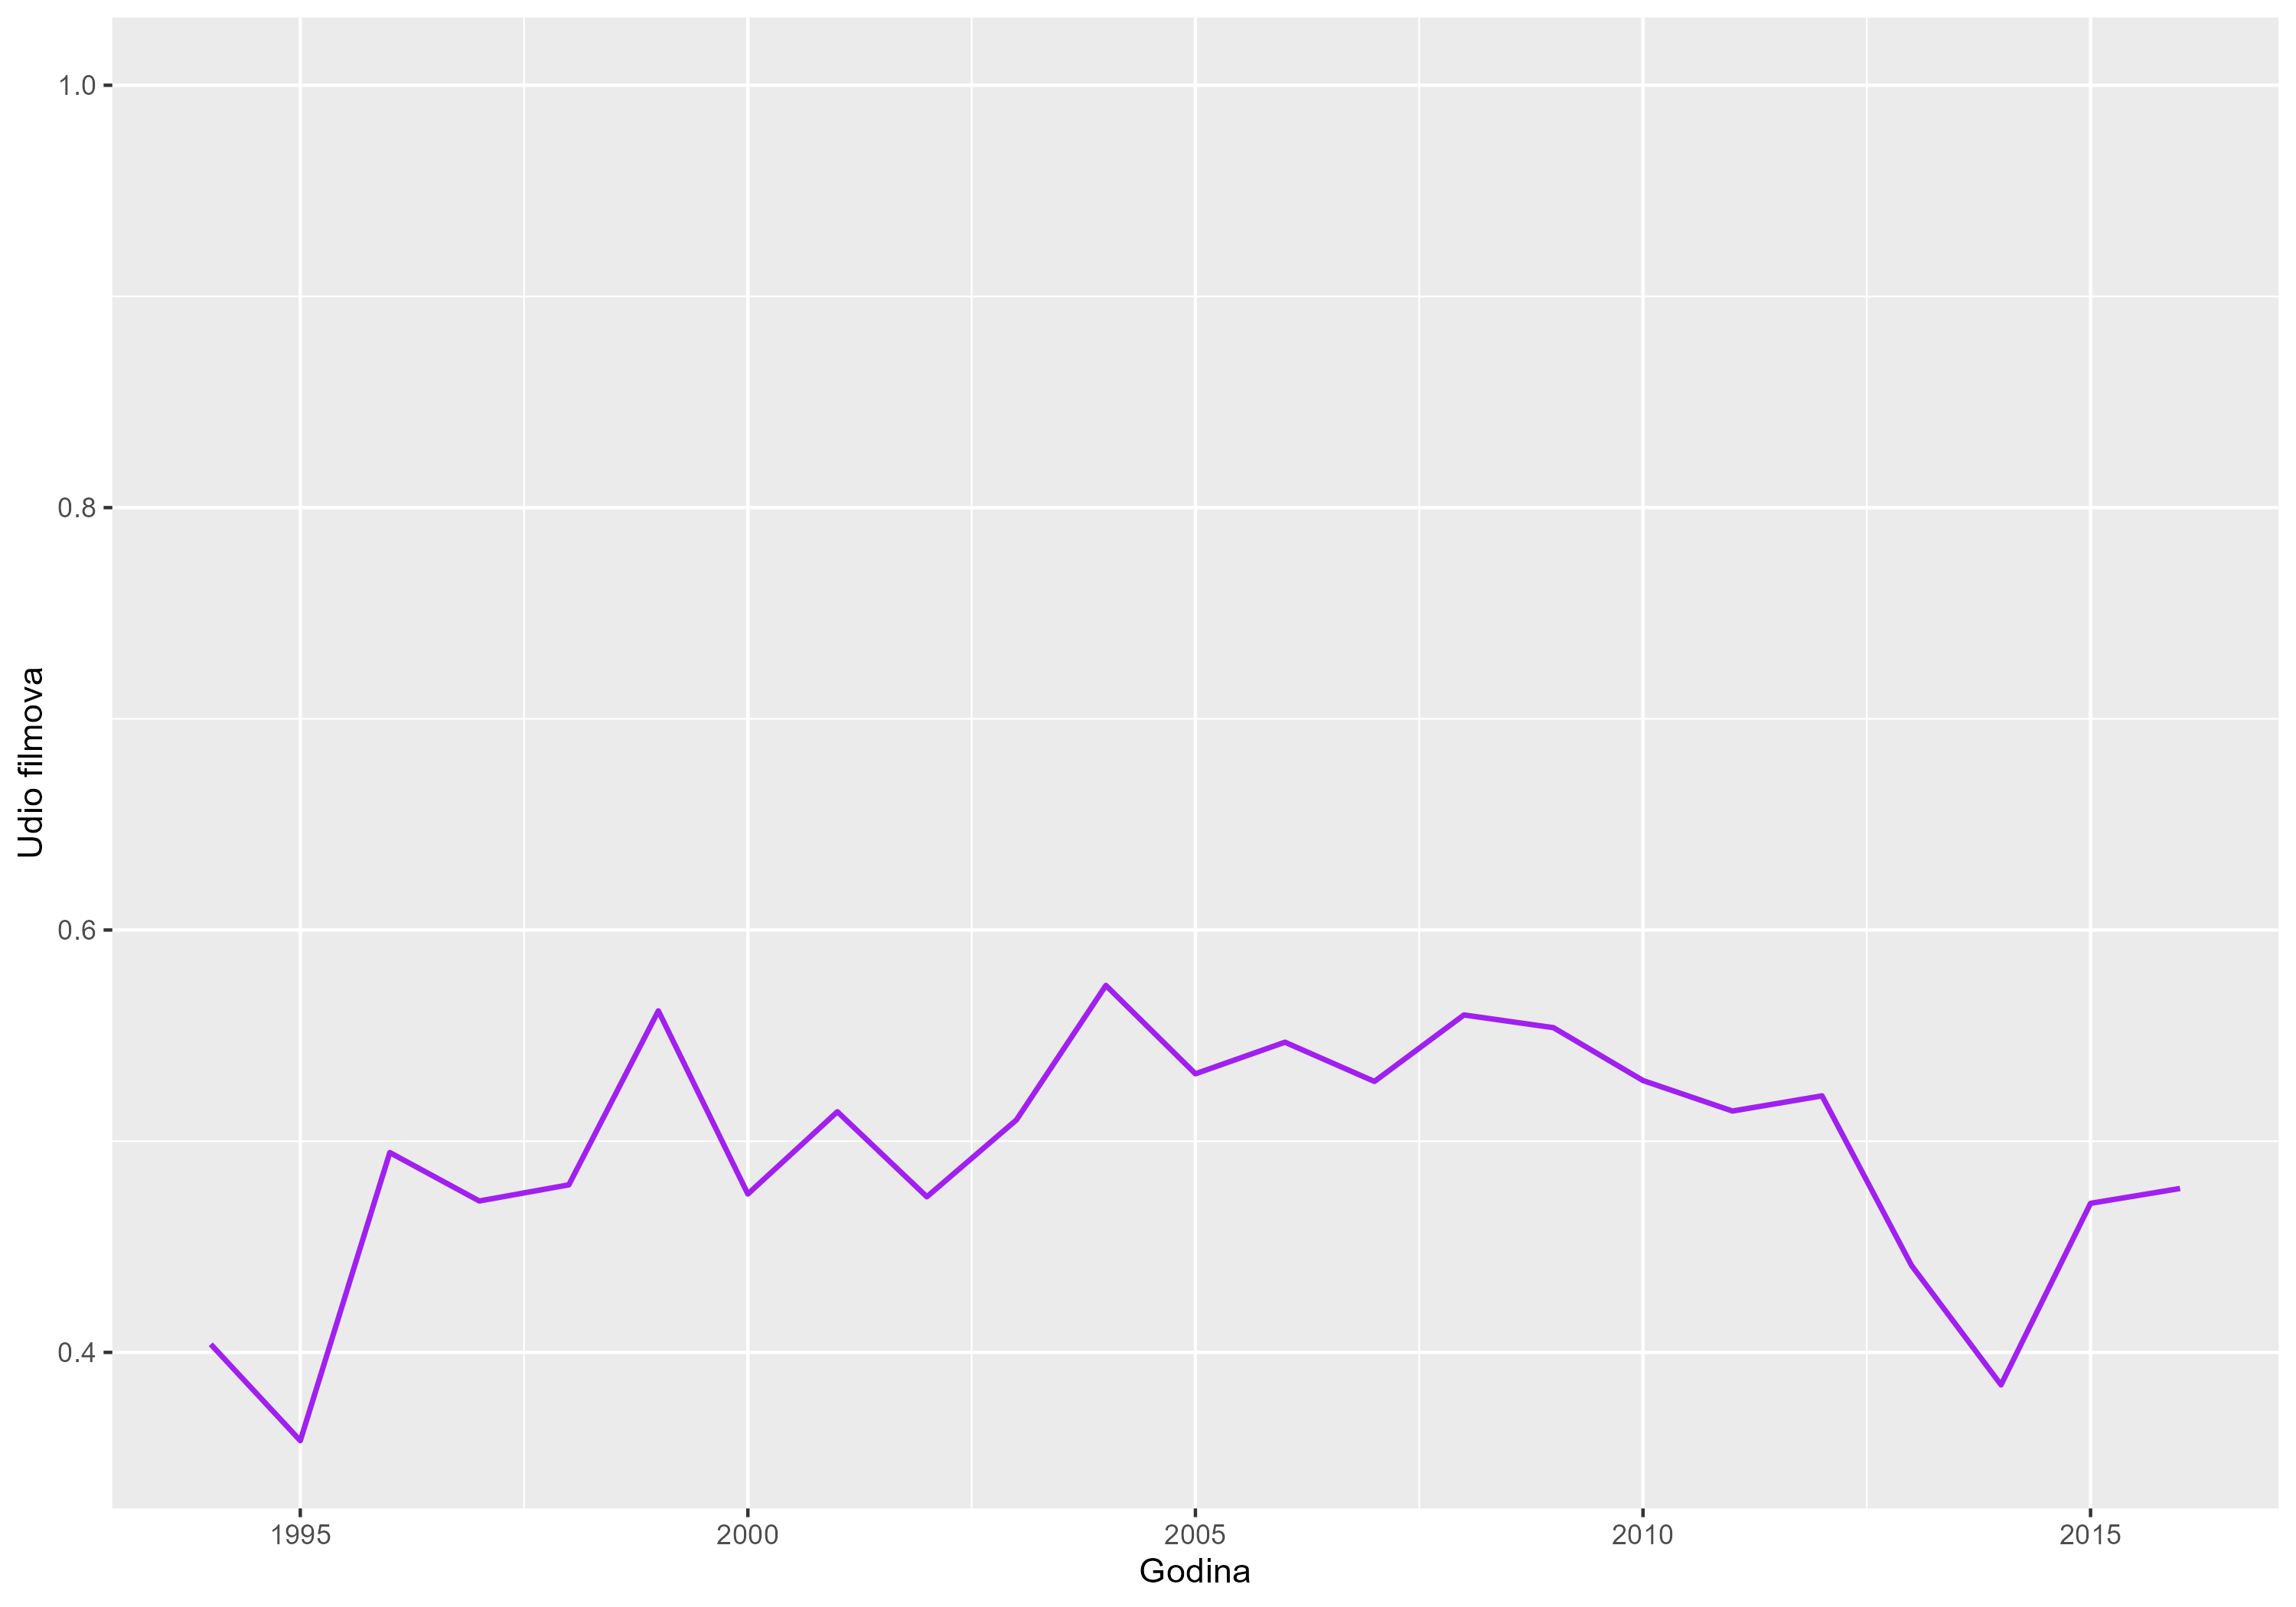
\includegraphics[width=15cm]{../figures/analysis/prihod_manji_od_budzeta.png}
	 	\caption{Postotak filmova koji su ostvarili manji prihoda od iznosa budžeta}
	 	\label{neuspjesno}
	 \end{figure}
	 
	 Stupac \texttt{duration} sadrži podatke o trajanju filmova. Najkraći film iz našeg skupa podataka traje 7, a najduži 511 minuta. Prosječno film traje 107 minuta. Histogram na slici \ref{trajanje} prikazuje broj filmova u ovisnosti o njihovom trajanju. 
	 
	  \begin{figure}[H]
	 	\centering
	 	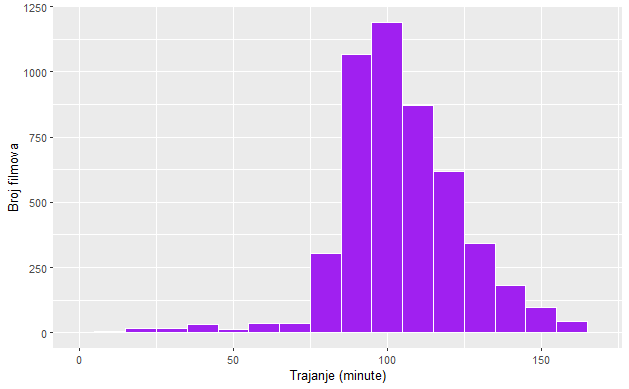
\includegraphics[width=15cm]{../figures/lucija_jednostavni/trajanje.png}
	 	\caption{Broj filmova po trajanju}
	 	\label{trajanje}
	 \end{figure}
	 
	 \begin{figure}[H]
	 	\centering
	 	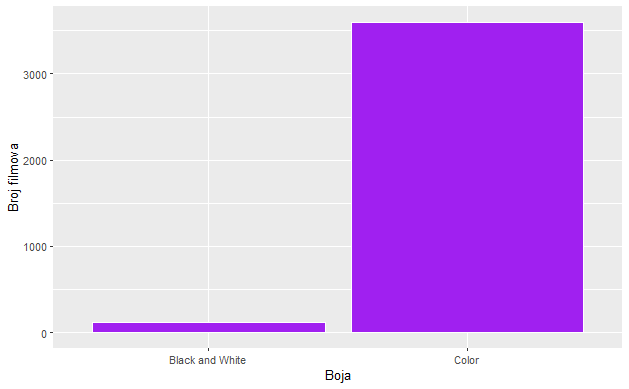
\includegraphics[width=15cm]{../figures/lucija_jednostavni/boja.png}
	 	\caption{Podjela filmova po boji}
	 	\label{boja}
	 \end{figure}
	 
	 \begin{figure}[H]
	 	\centering
	 	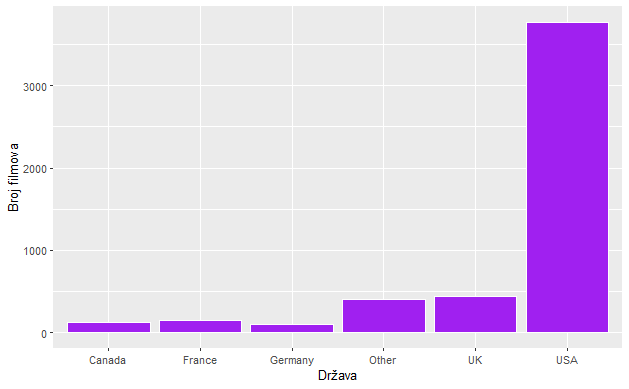
\includegraphics[width=15cm]{../figures/lucija_jednostavni/drzava.png}
	 	\caption{Podjela filmova po državi nastanka}
	 	\label{drzava}
	 \end{figure}
	 
	 \begin{figure}[H]
		 \centering
		 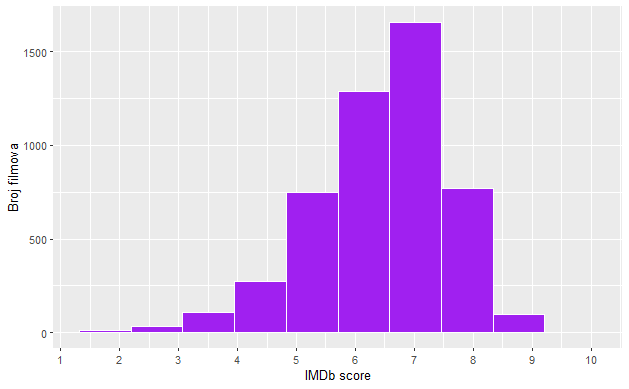
\includegraphics[width=15cm]{../figures/lucija_jednostavni/imdb.png}
		 \caption{Podjela filmova po uspješnosti}
		 \label{imdb}
	 \end{figure}
	 
	 \begin{figure}[H]
		 \centering
		 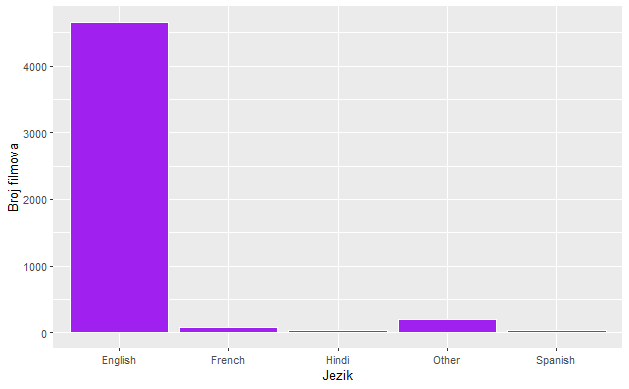
\includegraphics[width=15cm]{../figures/lucija_jednostavni/jezik.png}
		 \caption{Broj filmova s obzirom na jezik}
		 \label{jezik}
	 \end{figure}
	 
	
	 
	 
	 
	 
	 
	 
	 
	 
	\eject